\documentclass[11pt]{exam}
\newcommand{\myname}{Sihao Yin, Yuxuan Jiang} %Write your name in here

\newcommand{\myUCO}{0028234022, 0028440468} %write your UCO in here

\newcommand{\myhwtype}{Homework}
\newcommand{\myhwnum}{2} %Homework set number
\newcommand{\myclass}{CS580}
\newcommand{\mylecture}{}
\newcommand{\mysection}{}
\usepackage{listings}
% Prefix for numedquestion's
\newcommand{\questiontype}{Question}

% Use this if your "written" questions are all under one section
% For example, if the homework handout has Section 5: Written Questions
% and all questions are 5.1, 5.2, 5.3, etc. set this to 5
% Use for 0 no prefix. Redefine as needed per-question.
\newcommand{\writtensection}{0}

\usepackage{amsmath, amsfonts, amsthm, amssymb}  % Some math symbols
\usepackage{enumerate}
\usepackage{enumitem}
\usepackage{graphicx}
\usepackage{hyperref}
\usepackage[all]{xy}
\usepackage{wrapfig}
\usepackage{fancyvrb}
\usepackage[T1]{fontenc}
\usepackage{listings}

\usepackage{centernot}
\usepackage{mathtools}
\DeclarePairedDelimiter{\ceil}{\lceil}{\rceil}
\DeclarePairedDelimiter{\floor}{\lfloor}{\rfloor}
\DeclarePairedDelimiter{\card}{\vert}{\vert}


\setlength{\parindent}{0pt}
\setlength{\parskip}{5pt plus 1pt}
\pagestyle{empty}

\def\indented#1{\list{}{}\item[]}
\let\indented=\endlist

\newcounter{questionCounter}
\newcounter{partCounter}[questionCounter]

\newenvironment{namedquestion}[1][\arabic{questionCounter}]{%
    \addtocounter{questionCounter}{1}%
    \setcounter{partCounter}{0}%
    \vspace{.2in}%
        \noindent{\bf #1}%
    \vspace{0.3em} \hrule \vspace{.1in}%
}{}

\newenvironment{numedquestion}[0]{%
	\stepcounter{questionCounter}%
    \vspace{.2in}%
        \ifx\writtensection\undefined
        \noindent{\bf \questiontype \; \arabic{questionCounter}. }%
        \else
          \if\writtensection0
          \noindent{\bf \questiontype \; \arabic{questionCounter}. }%
          \else
          \noindent{\bf \questiontype \; \writtensection.\arabic{questionCounter} }%
        \fi
    \vspace{0.3em} \hrule \vspace{.1in}%
}{}

\newenvironment{alphaparts}[0]{%
  \begin{enumerate}[label=\textbf{(\alph*)}]
}{\end{enumerate}}

\newenvironment{arabicparts}[0]{%
  \begin{enumerate}[label=\textbf{\arabic{questionCounter}.\arabic*})]
}{\end{enumerate}}

\newenvironment{questionpart}[0]{%
  \item
}{}

\newcommand{\answerbox}[1]{
\begin{framed}
\vspace{#1}
\end{framed}}

\pagestyle{head}

\headrule
\header{\textbf{\myclass\ \mylecture\mysection}}%
{\textbf{\myname\ (\myUCO)}}%
{\textbf{\myhwtype\ \myhwnum}}

\begin{document}
\thispagestyle{plain}
\begin{center}
  {\Large \myclass{} \myhwtype{} \myhwnum} \\
  \myname{} (\myUCO{}) \\
  \today
\end{center}


%Here you can enter answers to homework questions

\begin{numedquestion}
   The following is the recursion tree\\
   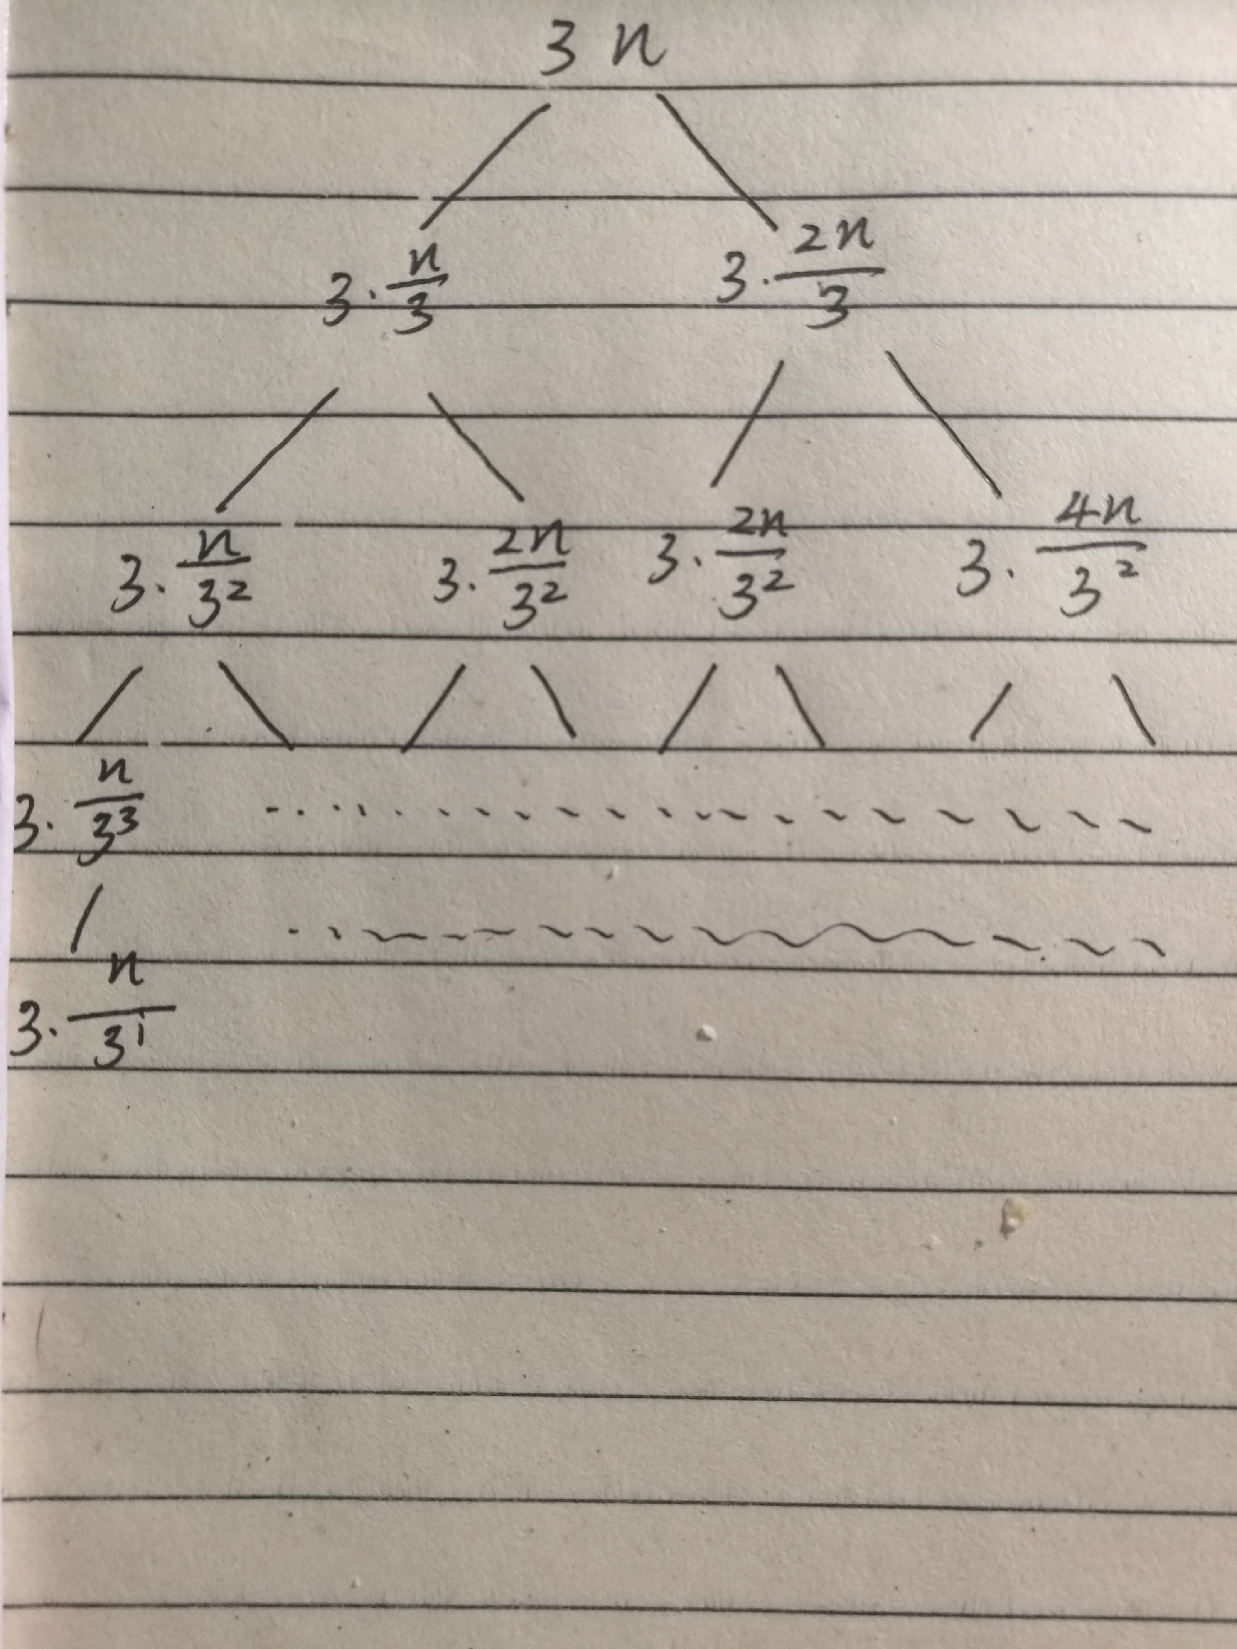
\includegraphics[scale=0.5]{images/fig1.pdf}\\
   Sum of the second level: 3n\\
   Sum of the third level: 3n\\ 
   Sum of the fourth level: 3n\\
   Height on the left subtree is $log_3^n$ and height on the right subtree is $log_\frac{3}{2}^n$. Clearly the right subtree is deeper.Since we are looking for an upper bound, we need to take this height\\
   Since the number of nodes at height k is $2^k$, the number of nodes at the base level should be $2^{log_{\frac{3}{2}}^n}$ = $n^{log_{\frac{3}{2}}^2}$. However, this is not a complete binary tree and leaves will be more and more absent in the bottom level, it will contribute less than cn to the cost \\
   Hence, T(n) <= 3n * $log_1.5^n$
   Hence T(n) = O(n*$log^n$)
   
%%%%%
  Let h be the height of the tree. Since $\frac{2n}{3} > \frac{n}{3}$, the $\frac{2n}{3}$ side of the tree will be the deepest branch. At the base level, $n(\frac{2}{3})^h = 1$, therefore, h = $log_\frac{3}{2}^n = log_{1.5}^n$. \\
  From the recurrence relation, we can see that the sum of cost of each level is always $(\frac{n}{3} + \frac{2n}{3}) * 3 = 3n$.\\
  Since the number of nodes at height k is  $2^k$, the number of nodes at the base level is $2^{log_{1.5}^n} = n^{log_{1.5}^2}$. \\
  Hence $T(n) <= \sum_{k=0}^{log_{1.5}^n-1}3n + 4.2*n^{log_{1.5}^2} = 
  O(n*log_{1.5}^n) + O(n^{log_{1.5}^2}) = O(n^{log_{1.5}^2})$. \\
   
\end{numedquestion}

\pagebreak
\begin{numedquestion}
  Below is the pseudocode, we use a max-heap of size K to achieve this. We loop through the input array A and see if the current element is smaller than the max in the max-heap. If it is, we put it in the array; if not, we move on. In the end, the k smallest elements will be contained in the heap\\\\
    \begin{lstlisting}
     
     function findKSmallest(A[1...N],k):
        H is a max-heap with size k
        put A[1] in the max-heap H 
        
        loop through A from 2 to N with index i:
            if A[i] < max in H:
                if H is full:
                    remove max
                put A[i] in the heap
        
        return H
        

    \end{lstlisting}

\textbf{Analysis:} 
\begin{enumerate}
    \item This alogirthm is correct because the max heap will always contain the biggest of the current k smallest elements and the heap will only take in elements that are smaller than the current max in the heap. Once the heap is full, we pop the biggest of the current k smallest elements. Hence the heap will always contain the k smallest elements.  
    \item From class, we know that the time complexity to insert an item to a heap is O(log k), with k being the size of the heap. The time complexity to pop or get the root the heap is O(1)
    \item Since we are iterating through the input array, in the worst case, we need to insert every item in the array to the heap. Hence, this algorithm is O(n*log k)
   
 
\end{enumerate}
      
\end{numedquestion}

\begin{numedquestion}
    \begin{enumerate}
        \item The following is the pseudocode 
    \begin{lstlisting}
        function partition(A[1..N],left,right):
            j = 1
            pick a random element p to be the pivot 
            loop through array A with index i from left to right:
                if A[i] <= p:
                    swap A[i] and A[j]
                    increment j
            swap A[j] and p 
            return j
            
        function find(A[1..N],left,right,k):
            if k is larger than the number of elements contained 
            between left and right:
                return NULL
                
            pos = partition(A[1..N],left,right)
                
            if pos is k:
                return A[pos]
                    
            else if pos > K:
                find(A[1...N],left,pos,k)
            else if pos < k:
                find(A[1...N],pos,right,k)
                
    \end{lstlisting}
        
        \item We demonstrate the algorithm expects to take O(n) time
        \begin{enumerate}
            \item We first define the indicator variable $X_k$ for k = 1 to N. $X_k$ = 1 if A[left,pos] contains exactly k elements. 
            
            \item Since the we partition the array to two parts, in order to compute the upper bound, we can assume our target resides in the larger part of the two parts 
            
            \item In function find, besides the recursive call, we also need to perform the partition, since we iterate the input array once in function partition, the time complexity is $\Theta(n)$
            \item Since whether we perform the recursive call depends on the value of $X_k$, we can write the recurrence as follows \\
                T(n) <= $\sum_{k=1}^n$ $X_k$ T(max(k-1,n-k)) + $\Theta(n)$
            \item Now we compute E(T(n)) \\
                \begin{enumerate}
                    \item E(T(n)) <= E($\sum_{k=1}^n$ $X_k$ T(max(k-1,n-k)) + $\Theta(n)$)
                    \item By linearity of expectation, E($\sum_{k=1}^n$ $X_k$ T(max(k-1,n-k)) + $\Theta(n)$) = $\sum_{k=1}^n$E( $X_k$ T(max(k-1,n-k))) + $\Theta(n)$
                    \item Since the choice of the pivot is independent in different recursive calls, we have $\sum_{k=1}^n$E( $X_k$ T(max(k-1,n-k))) + $\Theta(n)$ = $\sum_{k=1}^n$E($X_k$) * E(T(max(k-1,n-k))) + $\Theta(n)$
                    \item Since the pivot is selected uniformly random, E($X_k$) = $\frac{1}{n}$. Hence $\sum_{k=1}^n$E($X_k$) * E(T(max(k-1,n-k))) + $\Theta(n)$ = $\sum_{k=1}^n\frac{1}{n}$ * E(T(max(k-1,n-k))) + $\Theta(n)$ 
                    \item after a closer look, we can see we are summing up the time for arrays with the following pair of sizes (0,n-1), (1,n-2),...,(n-2,1),(n-1,0). Also, since max(k-1,n-k) = k-1 if k > $\floor{\frac{n}{2}}$ and = n - k if k < $\floor{\frac{n}{2}}$, each term from T($\floor{\frac{n}{2}}$) to T(n-1) has been repeated twice. Hence,$\sum_{k=1}^n\frac{1}{n}$ * E(T(max(k-1,n-k))) + $\Theta(n)$  = $\sum_{k=\floor{\frac{n}{2}}}^{n-1}\frac{2}{n}$ * E(T(k)) + $\Theta(n)$  
                    \item With the above, we demonstrate E(T(n)) is O(n) using substitution. 
                        \begin{enumerate}
                            \item If E(T(k)) is O(n), then E(T(k)) <= ck for some large constant c
                            \item We also replace $\Theta(n)$ with dn, for a constant d
                            \item Now, we have E(T(n)) <= $\frac{2}{n} \sum_{k=\floor{\frac{n}{2}}}^{n-1}ck$ + dn 
                            \item Note $\sum_{k=\floor{\frac{n}{2}}}^{n-1}ck$ = $\sum_1^{n-1}ck$ - $\sum_{k=\floor{\frac{n}{2}}-1}^{n-1}ck$ and $\sum_1^{a}k$ = $\frac{(a)(a+1)}{2}$, we have $\sum_{k=\floor{\frac{n}{2}}}^{n-1}ck$ = $\frac{(n-1)n}{2}$ - $\frac{(\floor{\frac{n}{2}}-1)\floor{\frac{n}{2}}}{2}$ <= $\frac{(n-1)n}{2}$ - $\frac{(\frac{n}{2}-2)(\frac{n}{2}-1)}{2}$
                            \item Hence, E(T(n)) <= $\frac{2}{n} \sum_{k=\floor{\frac{n}{2}}}^{n-1}ck$ + dn <= $\frac{2}{n}$($\frac{(n-1)n}{2}$ - $\frac{(\frac{n}{2}-2)(\frac{n}{2}-1)}{2}$ )+ dn
                            \item Therefore, with simplification, we have E(T(n)) <= cn - ($\frac{cn}{4} - \frac{c}{2}-dn$)
                            \item In order to finish the prove, we need to find a large enough n so that $\frac{cn}{4} - \frac{c}{2}-dn$ > 0. With some math, we can see that n>= $\frac{2c}{c-4a}$ 
                        \end{enumerate}
                    \item Hence, E(T(n)) is O(n)
                \end{enumerate}
            
            
        \end{enumerate}
    \end{enumerate}
\end{numedquestion}

% if you do not solve some of the questions use this command to increment counter
%\setcounter{questionCounter}{4}
%\begin{numedquestion}
%  Questions 2 and 3 were not solved, this is an answer to question 5.
%\end{numedquestion}


% if questions have subparts, use this command
%\pagebreak
%\begin{numedquestion}
%  Use the alphaparts environment to for letters.
%  \begin{alphaparts}
%    \item Part a
%    \item Part b
%    \item Part c
%  \end{alphaparts}
%\end{numedquestion}


%\begin{numedquestion}
%  Using the \texttt{description} environment is a great way to typeset induction proofs!
%  \begin{description}
%    \item[Base Case:]
%      Here I have my base case.
%    \item[Induction Hypothesis:]
%      Assume things to make proof work. 
%    \item[Induction Step:]
%      Prove all the things.
%  \end{description}

%  Therefore, we have proven the claim by induction on in the \texttt{description} environment.
%\end{numedquestion}



\end{document}
